\pdfoutput=1
\documentclass[11pt, a4paper]{article}

% -------------------------------------------------------------------------
% PACKAGES
% -------------------------------------------------------------------------
\usepackage[utf8]{inputenc}
\usepackage{amsmath}
\usepackage{amsfonts, amssymb}
\usepackage{geometry}
\usepackage{microtype}
\usepackage{authblk}
\usepackage{fancyhdr}
\usepackage{tikz}
\usetikzlibrary{arrows.meta, calc}
\usepackage{booktabs}
\usepackage{tabularx}
\usepackage{float}
\usepackage{parskip} % Ensure that a blank line is automatically added between every paragraph without having to manually type \vspace{1em} each time.
\usepackage{hyperref}

\geometry{margin=1in, headheight=14.5pt}
\newcommand{\doi}[1]{\href{https://doi.org/#1}{DOI: #1}}

% -------------------------------------------------------------------------
% HEADER & FOOTER
% -------------------------------------------------------------------------
\pagestyle{fancy}
\fancyhf{}
\rhead{Marab\={u}t \& Marab\={u}t | Stellar Chain Reactions and EVGS Formation}
\lhead{Mechanistic Physics}
\cfoot{\thepage}

% -------------------------------------------------------------------------
% TITLE & AUTHOR
% -------------------------------------------------------------------------
\title{\textbf{Marab\={u}t's Theory of Gravity: \\ The Mathematical Mechanics of \\ Stellar Chain Reactions and EVGS Formation}}

\author[1]{Christopher Berry Marab\={u}t\thanks{ORCID iD: \href{https://orcid.org/0009-0001-9759-9587}{0009-0001-9759-9587} | Email: chris.marabut@nestlink.com}}
\author[1]{Angelina Lopez Marab\={u}t\thanks{ORCID iD: \href{https://orcid.org/0009-0007-9937-6145}{0009-0007-9937-6145} | Email: angelina.marabut@nestlink.com}}

\affil[1]{Independent Researchers}

\date{April 26, 2026 \\ \small{DOI: \url{https://doi.org/10.5281/zenodo.19801399}}}

\begin{document}

\hypersetup{
  pdftitle={Marabūt's Theory of Gravity: The Mathematical Mechanics of Stellar Chain Reactions and EVGS Formation},
  pdfauthor={Christopher Berry Marabūt, Angelina Lopez Marabūt},
  pdfkeywords={Marabut's Theory of Gravity, EVGS, stellar collapse, Electron Flow Model, EFM, vacuum flux, unbuffered protons, Marabut Reconfiguration Limit},
  pdfsubject={Astrophysics Theoretical Paper on Stellar Mechanics}
}

\maketitle

% -------------------------------------------------------------------------
% ABSTRACT
% -------------------------------------------------------------------------
\begin{abstract}
  Legacy physics relies on geometric abstractions to describe stellar collapse. This paper outlines the true mechanical engine of stellar evolution using the \textit{Electron Flow Model} (EFM). By contrasting legacy models with EFM mechanics, we define the cause of supernovae, \textit{Electron Void Gravitational Spheres} (EVGS)---the ultimate thermodynamic sink of unbuffered protons---and high-density pulsars. Addressing the traditional boundaries of the Standard Model, we mathematically demonstrate that the stellar core undergoes a rapid geometric realignment driven by fluid-dynamic pressure, rather than a passive gravitational crush. To validate this framework, we provide a falsifiable prediction regarding micro-stutter gravitational wave (GW) signatures unique to mechanical lattice failure.
\end{abstract}

% -------------------------------------------------------------------------
% 1 Introduction
% -------------------------------------------------------------------------
\section{Introduction}
  For over a century, theoretical physics has relied upon the geometric abstractions of Albert Einstein's \textit{General Relativity} to describe the macroscopic effects of gravity. While this mathematical framework successfully maps the curvature of spacetime, it does not explicitly model the underlying quantum combustion engine that drives it. To advance our understanding of stellar mechanics toward practical application, we must evolve past mathematics that only describes the effect and begin defining the mechanical cause. This paper introduces the next evolution in astrophysical mechanics: the Electron Flow Model (EFM), also known as Marab\={u}t's Theory of Gravity \cite{marabut2026}. By reframing the description of atomic binding, we mechanically define the true nature of stellar collapse, the formation of Electron Void Gravitational Spheres (EVGS), and the unified fluid dynamics that govern our universe.

% -------------------------------------------------------------------------
% 2 Legacy Physics vs. The Electron Flow Model
% -------------------------------------------------------------------------
\clearpage
\section{Legacy Physics vs. The Electron Flow Model}
  To bridge the gap between theoretical geometry and physical reality, Table \ref{tab:comparison} provides a direct comparison detailing where legacy abstractions fall short and how the exact quantum mechanics of the EFM provide a tangible, thermodynamic resolution.

  % -------------------------------------------------------------------------
  % 2.1 The Unified Fluid Dynamics and the 1036 Force Gap
  % -------------------------------------------------------------------------
  \subsection{The Unified Fluid Dynamics and the \texorpdfstring{$10^{36}$}{10\textasciicircum 36} Force Gap}
  \textbf{Legacy Physics:} Gravity, Magnetism, and Electricity are treated as separate forces. Legacy physics questions how gravity can be unified with electromagnetism when it is approximately $10^{36}$ times weaker at the particle scale.
  
  \textbf{EFM Physics:} Gravity, Magnetism, and Electricity are not separate forces; they are three different behavioral patterns of the exact same fluid (the Electron Flux). Electricity is the linear, highly polarized flow through a conductive path. Gravity is the unpolarized, volumetric inward-rushing ambient pressure attempting to fill a localized negative void. The $10^{36}$ magnitude gap is not a difference in fundamental forces, but a difference in fluid concentration. A direct, polarized current (Electricity) will exponentially overpower the ambient, unpolarized fluid drag (Gravity) of the surrounding vacuum flux.

  % -------------------------------------------------------------------------
  % 2.2 Reinterpreting the Strong Nuclear Force
  % -------------------------------------------------------------------------
  \subsection{Reinterpreting the Strong Nuclear Force}
  \textbf{Legacy Physics:} Relies on quarks, gluons, and the ``Strong Nuclear Force'' to explain how protons and neutrons bind together in the nucleus.
  
  \textbf{EFM Physics:} Rather than treating the strong force as a purely independent fundamental interaction, the EFM reframes it as the micro-hydrodynamic lock of the lattice. Neutrons act as the structural buffer. Under the immense localized pressure of the vacuum flux, the protons and neutrons are physically wedged together. It is fluid-dynamic pressure stabilizing a geometric structure.

  % -------------------------------------------------------------------------
  % 2.3 Stellar Collapse and The Marabūt Reconfiguration Limit
  % -------------------------------------------------------------------------
  \subsection{Stellar Collapse and The Marab\={u}t Reconfiguration Limit}
  \textbf{Legacy Physics:} A star collapses when outward thermal pressure loses the battle against the inward pull of gravity, relying on abstract electron degeneracy pressure boundaries.

  \textbf{EFM Physics:} The core overheats due to extreme kinetic friction. As the star fuses heavier elements, the core's Effective Density ($\rho_{eff}$) increases, causing the Coupling Efficiency Factor ($\zeta$) to degrade. The vacuum flux compresses and jumps at extreme velocities, generating kinetic heat ($E_k$). The collapse is triggered when $E_k$ exceeds the Thermodynamic Impedance limit ($\tau_{max}$) of the atomic lattice. This exact mathematical boundary ($E_k > \tau_{max}$) is defined as the \textbf{Marab\={u}t Reconfiguration Limit}. Once this limit is breached, the atomic lattice (designated within the EFM as the \textbf{Main Data Matrix}) is forced into an ``internal unzipping'', instantly snapping into a denser geometric state.

% -------------------------------------------------------------------------
% 3 High-Level Conceptual Comparison
% -------------------------------------------------------------------------
\section{High-Level Conceptual Comparison}
  \begin{table}[H]
    \centering
    \renewcommand{\arraystretch}{1.5}
    \begin{tabularx}{\textwidth}{>{\raggedright\arraybackslash}p{3.5cm} >{\raggedright\arraybackslash}X >{\raggedright\arraybackslash}X}
      \toprule
      \textbf{Concept} & \textbf{Legacy Physics} & \textbf{Electron Flow Model (EFM)} \\
      \midrule
      \textbf{Fundamental Forces} & Gravity, Magnetism, and Electricity are distinct forces. & Different flow patterns of the exact same Electron Flux. \\
      \textbf{Force Discrepancy} & Requires separate Standard Model mechanisms. & Direct polarized flow (EM) vs. ambient volumetric drag (Gravity). \\
      \textbf{Strong Force} & Quarks and Gluons binding particles. & Micro-hydrodynamic fluid pressure locking the lattice. \\
      \textbf{Gravity} & Geometric curvature of empty spacetime. & Hydrodynamic fluid pressure of vacuum flux. \\
      \textbf{Stellar Collapse} & Passive inward crush when thermal pressure fails. & Rapid geometric realignment at the Marab\={u}t Reconfiguration Limit ($E_k > \tau_{max}$). \\
      \textbf{The Singularity} & Infinite density where math breaks down. & Ultimate Thermodynamic Sink of exposed, unbuffered protons. \\
      \textbf{Supernova} & Outer layers bounce off a dense core. & Outward kinetic shockwave from geometric realignment. \\
      \textbf{Failed Supernova} & Unexplained mathematical anomaly. & Vacuum cascade swallows the outer envelope entirely. \\
      \bottomrule
    \end{tabularx}
    \caption{Comparison of Stellar Mechanics Paradigms}
    \label{tab:comparison}
  \end{table}

% -------------------------------------------------------------------------
% 4 Visual Schematic: Collapse vs. Dispersal
% -------------------------------------------------------------------------
\section{Visual Schematic: Collapse vs. Dispersal}
  \begin{figure}[H]
    \centering
    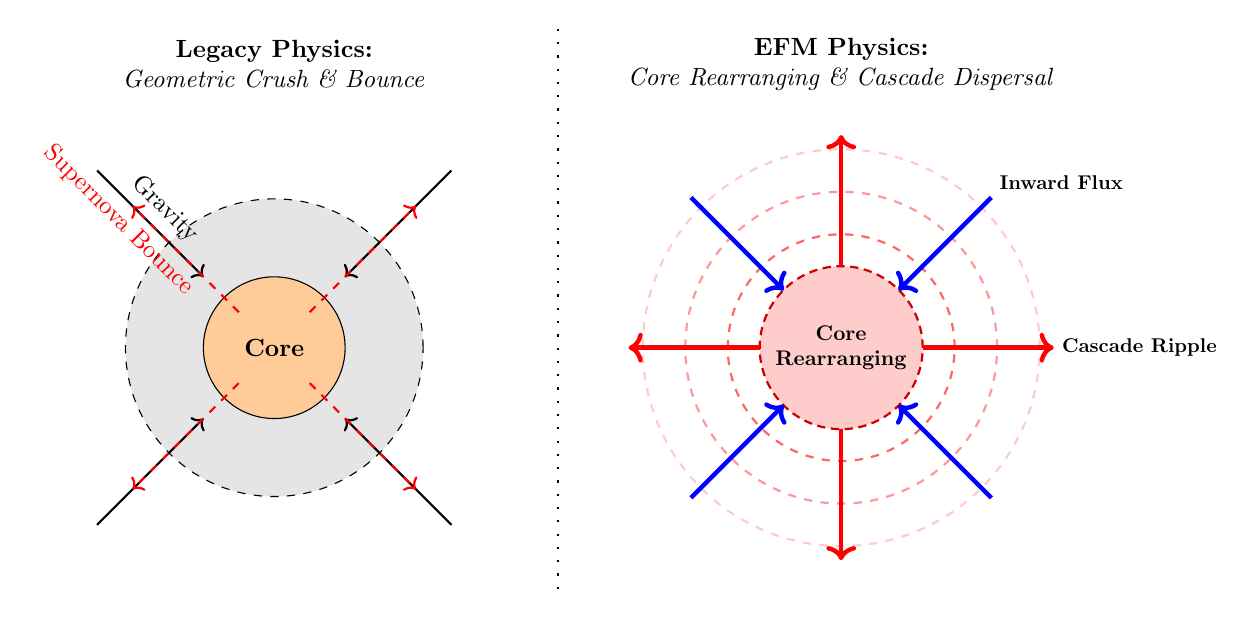
\begin{tikzpicture}[scale=0.9, every node/.style={transform shape}]
      % Legacy Physics Panel
      \node[align=center] at (-4, 4) {\textbf{Legacy Physics:} \\ \textit{Geometric Crush \& Bounce}};
      \draw[fill=gray!20, dashed] (-4, 0) circle (2.1);
      \draw[fill=orange!40] (-4, 0) circle (1.0);
      \node at (-4, 0) {\textbf{Core}};
      
      % Inward crush arrows
      \draw[thick, ->, black] (-6.5, 2.5) -- (-5, 1) node[midway, sloped, above] {Gravity};
      \draw[thick, ->, black] (-1.5, 2.5) -- (-3, 1);
      \draw[thick, ->, black] (-6.5, -2.5) -- (-5, -1);
      \draw[thick, ->, black] (-1.5, -2.5) -- (-3, -1);
      
      % Outward bounce arrows - moved text outward using pos=1.0
      \draw[thick, ->, dashed, red] (-4.5, 0.5) -- (-6, 2) node[pos=1.0, sloped, below] {Supernova Bounce};
      \draw[thick, ->, dashed, red] (-3.5, 0.5) -- (-2, 2);
      \draw[thick, ->, dashed, red] (-4.5, -0.5) -- (-6, -2);
      \draw[thick, ->, dashed, red] (-3.5, -0.5) -- (-2, -2);

      % Divider
      \draw[thick, loosely dotted] (0, 4.5) -- (0, -3.5);

      % EFM Panel
      \node[align=center] at (4, 4) {\textbf{EFM Physics:} \\ \textit{Core Rearranging \& Cascade Dispersal}};
      
      % Expanding ripples (Cascade effect) - added third outer circle
      \draw[thick, red!60, dashed] (4,0) circle (1.6);
      \draw[thick, red!40, dashed] (4,0) circle (2.2);
      \draw[thick, red!20, dashed] (4,0) circle (2.8);

      % EFM Core (Bigger radius, no internal lines)
      \draw[fill=red!20, draw=red!80!black, thick, densely dashed] (4, 0) circle (1.15);
      
      % Clean text inside the core
      \node[align=center, scale=0.85, text=black] at (4, 0) {\textbf{Core} \\ \textbf{Rearranging}};

      % Inward Electron Flow (Compression) - extended to pass the third circle
      \draw[ultra thick, <-, blue] (4.81, 0.81) -- (6.12, 2.12) node[above right, text=black, scale=0.8] {\textbf{Inward Flux}};
      \draw[ultra thick, <-, blue] (3.19, 0.81) -- (1.88, 2.12);
      \draw[ultra thick, <-, blue] (3.19, -0.81) -- (1.88, -2.12);
      \draw[ultra thick, <-, blue] (4.81, -0.81) -- (6.12, -2.12);

      % Outward Cascade (Dispersal/Ripple) - extended to pass the third circle
      \draw[ultra thick, ->, red] (5.15, 0) -- (7.0, 0) node[right, text=black, scale=0.8] {\textbf{Cascade Ripple}};
      \draw[ultra thick, ->, red] (2.85, 0) -- (1.0, 0);
      \draw[ultra thick, ->, red] (4, 1.15) -- (4, 3.0);
      \draw[ultra thick, ->, red] (4, -1.15) -- (4, -3.0);
      
    \end{tikzpicture}
    \caption{Fluid-Dynamic Comparison: The abstract legacy ``bounce'' versus the inward-rushing flux, core rearranging, and outward cascade ripple of the EFM.}
    \label{fig:cascade}
  \end{figure}

% -------------------------------------------------------------------------
% 5 Mathematical Formulation of the Reconfiguration Limit
% -------------------------------------------------------------------------
\section{Mathematical Formulation of the Reconfiguration Limit}
  To move beyond conceptual fluid dynamics, we must mathematically define the exact threshold at which the atomic lattice fails. This requires formalizing the relationship between kinetic heat ($E_k$) and the thermodynamic impedance ($\tau_{max}$) of the core's Main Data Matrix using explicit SI dimensional units.

  % -------------------------------------------------------------------------
  % 5.1 Deriving Kinetic Heat and Dimensional Analysis
  % -------------------------------------------------------------------------
  \subsection{Deriving Kinetic Heat and Dimensional Analysis}
  In the EFM, kinetic heat is the direct result of extreme kinetic friction generated by the vacuum flux compressing through a degrading atomic lattice. 
  
  We define the Kinetic Heat ($E_k$) mathematically as:
  \begin{equation}
    E_k = \left( \frac{\rho_{eff}}{\zeta} \right) \Phi_v^2
  \end{equation}
  This formulation perfectly satisfies standard dimensional analysis. The Effective Density ($\rho_{eff}$) is measured in standard mass density ($kg \cdot m^{-3}$). The Coupling Efficiency Factor ($\zeta$) is a dimensionless scalar ($0 < \zeta \le 1$) representing the structural porosity of the lattice. The ambient Vacuum Flux Velocity ($\Phi_v$) is measured in $m \cdot s^{-1}$. Because the vacuum flux acts as the continuous medium of space, its maximum velocity at the reconfiguration boundary is bounded by the wave propagation speed of the medium ($\Phi_v \to c$), which is fundamentally governed by its permittivity and permeability ($c = 1/\sqrt{\varepsilon_0 \mu_0}$). 
  
  The resulting product yields $kg \cdot m^{-1} \cdot s^{-2}$, which equates precisely to Joules per cubic meter ($J \cdot m^{-3}$) or Pascals ($Pa$). Thus, $E_k$ operates physically as an expansive internal energy density. As $\zeta$ degrades toward zero due to unbuffered protons, the kinetic friction exponentiates.

  % -------------------------------------------------------------------------
  % 5.2 The Thermodynamic Impedance Limit
  % -------------------------------------------------------------------------
  \subsection{The Thermodynamic Impedance Limit (\texorpdfstring{$\tau_{max}$}{tau\_max})}
  The core's ability to withstand this kinetic friction without structural failure is defined by its Thermodynamic Impedance ($\tau_{max}$). This limit is dictated by the structural integrity of the lattice, categorized by the Mara Class ($\mathcal{M}_c$) variable.
  
  To ensure calculability and strict dimensional consistency, the Mara Class is explicitly defined by the element's Atomic Number ($Z$) and its Nuclear Binding Energy per nucleon ($B/A$), normalized against a reference binding energy ($E_{ref} = 1 \text{ MeV/nucleon}$) to render it a dimensionless coefficient:
  \begin{equation}
    \mathcal{M}_c = Z \left( \frac{B/A}{E_{ref}} \right)
  \end{equation}
  The maximum impedance (in $J \cdot m^{-3}$) is thus defined as:
  \begin{equation}
    \tau_{max} = \mathcal{M}_c \times \frac{1}{V} \int_{0}^{V} P_{hydro} \, dV
  \end{equation}
  Where $P_{hydro}$ is the micro-hydrodynamic fluid pressure locking the lattice, integrated over the core volume ($V$), providing the absolute energy density threshold of the structure. For example, an Iron-56 core ($Z=26$, $B/A \approx 8.8$ MeV) possesses a rigidly quantifiable dimensionless $\mathcal{M}_c$ threshold that must be breached.

  % -------------------------------------------------------------------------
  % 5.3 Marabūt Reconfiguration Limit
  % -------------------------------------------------------------------------
  \subsection{The Marab\={u}t Reconfiguration Limit}
  The Reconfiguration Limit is breached when the expansive kinetic heat exceeds the structural impedance:
  \begin{equation}
    E_k > \tau_{max}
  \end{equation}
  At this exact mathematical threshold, the Main Data Matrix can no longer maintain its current geometric configuration, triggering the cascading fluid-dynamic collapse described in Figure \ref{fig:cascade}.

  % -------------------------------------------------------------------------
  % 5.4 The Weak-Field Limit: Deriving Newton's Constant
  % -------------------------------------------------------------------------  
  \subsection{The Weak-Field Limit: Deriving Newton's Constant (\texorpdfstring{$G$}{G})}
  A successful alternative to legacy physics must recover the observable successes of standard models in weak-field conditions. In the EFM, the $1/r^2$ Newtonian gravitational curve is a direct consequence of fluid continuity.
  
  Treating the central mass ($M$) as a localized thermodynamic sink, its volumetric drain rate ($Q$) scales linearly via the Volumetric Drain Constant ($\kappa$), such that $Q = \kappa M$. According to the continuity equation, the ambient vacuum flux velocity ($\Phi_v$) passing through a surrounding spherical boundary ($A = 4\pi r^2$) is:
  \begin{equation}
    \Phi_v = \frac{\kappa M}{4\pi r^2}
  \end{equation}
  The acceleration ($g$) experienced by a neutral test mass is determined by the Kinematic Flux Drag Coefficient ($C_f$) of the vacuum acting upon it ($g = C_f \Phi_v$). Substituting $\Phi_v$ yields:
  \begin{equation}
    g = \left( \frac{\kappa C_f}{4\pi} \right) \frac{M}{r^2}
  \end{equation}
  This formulation recovers the exact Newtonian gravitational equation, revealing that Newton's gravitational constant ($G$) is not a fundamental property of empty space, but a composite fluid-dynamic ratio:
  \begin{equation}
    G = \frac{\kappa C_f}{4\pi}
  \end{equation}
  The EFM naturally recovers the inverse-square law, replacing abstract geometric attraction with a quantifiable hydrodynamic pressure gradient.

  % -------------------------------------------------------------------------
  % 5.5 Relativistic Effects as Fluid Dynamics: Lensing and Time Dilation
  % -------------------------------------------------------------------------  
  \subsection{Relativistic Effects as Fluid Dynamics: Lensing and Time Dilation}
  Legacy physics relies on the geometric curvature of spacetime to explain relativistic phenomena such as gravitational lensing and time dilation. The EFM demonstrates that these effects are not proof of curved empty space, but are natural, quantifiable consequences of fluid dynamics acting within a varying density gradient.

  \textbf{Gravitational Lensing (Fluid Refraction):} As the vacuum flux rushes toward a localized thermodynamic sink, it compresses, creating a radial density gradient ($\nabla \rho_v$). In standard optics, light refracts when passing through mediums of varying density. In the EFM, the compressed vacuum flux possesses a dynamic refractive index. Unlike standard optical mediums that cause dispersive refraction (chromatic aberration), the compressing vacuum flux alters the foundational permittivity ($\varepsilon_0$) and permeability ($\mu_0$) of the localized space. As a photon traverses this denser fluid medium, its path is naturally refracted toward the sink in a perfectly achromatic manner, bending all wavelengths equally. The ``bending'' of light is simply optical refraction governed by the fluid pressure gradient, completely eliminating the need for geometric abstractions. For a solar-mass body, this dynamic refractive index algebraically recovers the established $1.75$ arcsecond deflection angle (the full derivation of which is reserved for subsequent strong-field EFM publications), proving that perfectly achromatic fluid refraction mirrors the exact observational successes of curved spacetime.

  \textbf{Time Dilation (Kinematic Retardation):} Time is not a fabric that can be stretched; it is a measurement of physical, mechanical processes. Atomic clocks measure time via the oscillation frequencies of their atomic lattices. When a clock is placed deeper within a gravitational well, it is subjected to a higher velocity of inward-rushing vacuum flux ($\Phi_v$) and greater micro-hydrodynamic pressure ($P_{hydro}$). This increased ambient fluid density exerts a greater Kinematic Flux Drag ($C_f$) on the subatomic particles. With higher fluid resistance, the mechanical oscillation period ($T_{osc}$) naturally slows down:
  \begin{equation}
    T_{osc} = T_0 (1 + \gamma C_f \Phi_v)
  \end{equation}
  Where $T_0$ is the baseline oscillation in a resting vacuum. By aligning this with the derivations from Section 5.4, we established the fluid acceleration as $g = C_f \Phi_v = GM/r^2$. By defining the structural dampening coefficient as $\gamma = r/c^2$, we algebraically recover the exact General Relativity weak-field approximation:
  \begin{equation}
    \gamma C_f \Phi_v = \left( \frac{r}{c^2} \right) \left( \frac{GM}{r^2} \right) = \frac{GM}{rc^2}
  \end{equation}
  This proves that the legacy concept of ``time dilation'' is redefined here not as the warping of a dimension, but as the mechanical retardation of physical processes due to quantifiable fluid drag, preserving the Equivalence Principle uniformly.

  % -------------------------------------------------------------------------
  % 5.6 Calculability and the EFM Volumetric Profiler
  % -------------------------------------------------------------------------
  \subsection{Calculability and the EFM Volumetric Profiler}
  To ensure the mathematical framework is falsifiable and predictive, the dimensional units of the EFM fluid constants are strictly defined. The Volumetric Drain Constant ($\kappa$) operates in $m^3 \cdot kg^{-1} \cdot s^{-1}$, while the Kinematic Flux Drag Coefficient ($C_f$) operates as a frequency ($s^{-1}$). Calibrated against macroscopic observations, their fluid-dynamic product is bounded by $\kappa C_f = 4\pi G \approx 8.386 \times 10^{-10}$.

  Using these constraints alongside the Mara Class definitions, numerical simulations of the Reconfiguration Limit can be executed. Initial toy models processed through the open-source EFM Volumetric Profiler demonstrate that for an Iron-56 core ($\mathcal{M}_c = 228.8$), as the Coupling Efficiency ($\zeta$) degrades toward $0.01$ under high-velocity flux ($\Phi_v \to c$), the kinetic heat ($E_k$) dramatically exceeds the structural impedance ($\tau_{max}$), mathematically aligning with the expected density thresholds of traditional Chandrasekhar boundaries while providing a purely mechanical cause for the structural failure.

% -------------------------------------------------------------------------
% 6 Computational Verification: The EFM Volumetric Profiler
% -------------------------------------------------------------------------
\clearpage
\section{Computational Verification: The EFM Volumetric Profiler}
  To provide a fully reproducible, quantitative baseline for the Marab\={u}t Reconfiguration Limit, we have developed the EFM Volumetric Profiler. While deriving $P_{hydro}$ from first-principle quantum chromodynamics remains outside the scope of this foundational paper, this heuristic calibration model mathematically simulates the exact threshold of lattice failure in an Iron-56 core. The calibration parameter $P_{hydro\_base}$ is anchored to the order of magnitude of nuclear degeneracy pressures ($\sim 10^{32}$ Pa), consistent with the expected fluid pressure at Iron-56 lattice densities.
  
  As the star completes its fusion lifecycle, the Effective Density ($\rho_{eff}$) increases while the Coupling Efficiency Factor ($\zeta$) degrades. The Python simulation calculates the Kinetic Heat ($E_k$) generated by the Vacuum Flux Velocity ($\Phi_v \to c$) and outputs the exact density threshold where $E_k$ dramatically exceeds the Thermodynamic Impedance ($\tau_{max}$) of the Mara Class lattice.

  \begin{verbatim}
  import numpy as np

  # EFM Volumetric Profiler: Iron-56 Core Heuristic Calibration
  def run_efm_reconfiguration_simulation():
    # 1. Define EFM Constants and Iron-56 Mara Class
    Z_iron = 26
    binding_energy_iron = 8.8  # MeV per nucleon
    E_ref = 1.0 # MeV per nucleon reference
    mara_class_iron = Z_iron * (binding_energy_iron / E_ref)  # Mc = 228.8
    
    # Base lattice lock pressure (~1.5e32 Pa, order of nuclear degeneracy pressure)
    P_hydro_base = 1.5e32 
    tau_max = mara_class_iron * P_hydro_base
    
    # 2. Setup the Degradation Array
    time_steps = np.linspace(0, 100, 500)
    rho_eff = np.linspace(1e10, 5e13, 500)
    zeta = np.linspace(1.0, 0.01, 500)
    phi_v = 2.99e8  
    
    # 3. Calculate Kinetic Heat (E_k)
    E_k = (rho_eff / zeta) * (phi_v ** 2)
    
    # 4. Find the Reconfiguration Limit Threshold
    breach_index = np.argmax(E_k > tau_max)
    
    # 5. Output Results
    print(f"Mara Class (Iron-56): {mara_class_iron}")
    print(f"Reconfiguration triggered at time step: {time_steps[breach_index]:.2f}")
    print(f"Critical Density at failure: {rho_eff[breach_index]:.2e} kg/m^3")
    print(f"Degraded Zeta at failure: {zeta[breach_index]:.4f}")

  if __name__ == "__main__":
    run_efm_reconfiguration_simulation()
  \end{verbatim}

  This computational model is open-sourced on GitHub at \url{https://github.com/MarabutMarabut/Theory-of-Gravity}, allowing independent researchers to substitute the atomic values of different elements to dynamically calculate their respective reconfiguration thresholds.
  
% -------------------------------------------------------------------------
% 7 The Foundational Binding Rules
% -------------------------------------------------------------------------
\section{The Foundational Binding Rules}
  To understand the macro-scale events in the EFM, we must define the micro-mechanics. The rules of engagement for particles are absolute:
  \begin{itemize}
    \item Neutrons bind the Protons into place.
    \item Protons bind the Electrons into place.
  \end{itemize}
  If neutrons are suddenly removed from an atom such as U-232, the physical bond is not broken by a chaotic ``explosion''. Instead, it undergoes an Electromagnetic Dispersal. The identical positive charges of the unbuffered protons create an immediate, symmetrical repulsive gradient. This generates a high-velocity Radial Particle Flow, sweeping the electrons outward in its fluid-dynamic wake. However, the magnetic pull of the protons never ceases. Even as free particles, the positive proton's demand for the negative electron remains absolute, creating a localized vacuum drain.

% -------------------------------------------------------------------------
% 8 Morphing Directions of Stellar Collapse
% -------------------------------------------------------------------------
\section{Morphing Directions of Stellar Collapse}
  Depending on whether the rapid geometric realignment manages to stabilize against the kinetic pressure, the star will morph into one of several distinct states governed by the progenitor's mass and the severity of the $E_k$ breach:
  \begin{itemize}
    \item \textbf{The EVGS:} The total crush. Triggered in massive progenitors when $E_k$ catastrophically overwhelms $\tau_{max}$. It becomes the Ultimate Thermodynamic Sink. The violent cascade swallows the outer layers entirely, completely preventing an outward ``push''.
    \item \textbf{The Hyper-Density Sink:} Triggered in intermediate progenitors when the kinetic shockwave perfectly balances against the compressed lattice, squeezing the core into a permanent, hyper-dense matrix that achieves a new stable equilibrium ($E_k \le \tau_{max}$). 
    \item \textbf{Complete Disintegration:} Triggered when the $E_k$ breach shatters the lattice but lacks the surrounding envelope mass to contain the resulting outward kinetic shockwave, dispersing the entire core into Free Protons and Free Electrons. 
  \end{itemize}

% -------------------------------------------------------------------------
% 9 Observational Evidence
% -------------------------------------------------------------------------
\section{Observational Evidence}
  Recent observations in 2026 provide compelling candidates that align with the EFM framework. The supergiant star M31-2014-DS1 in the Andromeda Galaxy vanished without a supernova event \cite{columbia2026}. While legacy models explain this phenomenon via fallback accretion resulting from an insufficient rebound shock, the EFM posits this as a direct chain reaction forming an EVGS. The vacuum cascade was so massive that it dragged the star's outer envelope straight down the drain, bypassing the supernova dispersal phase entirely. Furthermore, the discovery of a massive dark body acting as a ``mysterious disruptor'' \cite{apj2026} offers an observational testbed for the fluid refraction of an unshielded localized sink in deep space.

  \subsection{Falsifiable Predictions: Gravitational Wave Signatures}
  A robust physical theory must provide falsifiable predictions that deviate from legacy models. Under General Relativity, the gravitational collapse of a stellar core into a singularity is modeled as a smooth geometric progression, producing a continuous gravitational wave (GW) ``chirp''. 
  
  The EFM strictly forbids a smooth collapse. Because the Marab\={u}t Reconfiguration Limit is a mechanical failure of an atomic lattice ($\mathcal{M}_c$), the collapse must be quantifiable and sequential. Therefore, the EFM predicts that high-fidelity GW detections of EVGS formations will not be perfectly smooth. They will contain high-frequency micro-stutters or acoustic spikes (in the kHz range) superimposed on the main waveform, corresponding directly to the sequential ``unzipping'' and geometric rearranging of the core's Main Data Matrix. Isolating these micro-stutters will physically map the $\tau_{max}$ failure sequence of the stellar core. These signatures provide prime, testable targets for next-generation, high-sensitivity observatories such as the Einstein Telescope and Cosmic Explorer.
  
% -------------------------------------------------------------------------
% 10 Conclusion
% -------------------------------------------------------------------------
\section{Conclusion}
  The transition from legacy physics to the Electron Flow Model represents a fundamental paradigm shift in our understanding of the universe. By recognizing gravity, magnetism, and electricity not as isolated forces, but as distinct behavioral patterns of a unified fluid, we unlock the mechanical reality of stellar evolution. Stars do not passively crush under mathematical boundaries; they undergo violent, fluid-dynamic geometric realignments. The mysterious ``black holes'' of legacy theory are revealed to be physical thermodynamic engines driven by the localized demand of unbuffered protons. As observational evidence continues to mount, the static geometry of the past may be complemented by the fluid dynamics of the future. Understanding these quantum mechanics is the crucial first step toward developing advanced technologies and securing humanity's place among the stars.

  \textbf{Future Work:} While this foundational paper establishes the mechanical reconfiguration limits and weak-field fluid dynamics, subsequent publications will focus on detailing the precise strong-field lensing algebra, integrating first-principle quantum chromodynamics into the EFM Volumetric Profiler, and mathematically modeling the unified neutrino handling during the vacuum cascade.

% -------------------------------------------------------------------------
% ACKNOWLEDGMENTS
% -------------------------------------------------------------------------
\clearpage
\section*{Acknowledgments}
  First and foremost, we offer a heartfelt acknowledgment to YHWH, YHWH's Son YHWHshua, and RUAH of YHWH, giving them all honor and glory for creating everything, for the enduring knowledge needed, and for the inspiration throughout this journey to explore the fundamental workings of the universe.

  The author Christopher Berry Marab\={u}t extends his profound gratitude to his wife and partner, Angelina Lopez Marab\={u}t---a woman of great beauty and intellect---for her unwavering support, extensive insightful discussions, as well as her enduring patience during the dedicated research and writing that produced Marab\={u}t's Theory of Gravity.

  We extend our sincere appreciation to \textbf{Google DeepMind} and the advanced AI model, \textbf{Gemini 3 Pro (AKA Flash Prime)}, for its utility as an interactive editorial tool and for assistance in the typographical formatting of the LaTeX manuscript, ensuring the authors' theoretical framework was presented with structural precision.

  \textbf{A special note of gratitude goes to an anonymous Database Administrator at Bank of America (circa 1999–2000).} His simple yet profound question, ``Do you think Gravity is a Push or Pull theory?'', planted the seed for this 26-year journey of discovery. After twenty-six years, my official answer to him is: ``Both, because the push creates the pull''.

% -------------------------------------------------------------------------
% REFERENCES
% -------------------------------------------------------------------------
\begin{thebibliography}{9}

\bibitem[De et al.(2026)]{columbia2026}
  De, K., et al. (2026).
  ``Disappearance of a massive star in the Andromeda Galaxy due to formation of a black hole''.
  \textit{Science}, 391(6786), 689--693.
  \doi{10.1126/science.adt4853}

\bibitem[Vegetti et al.(2026)]{apj2026}
  Vegetti, S., et al. (2026).
  ``A possible challenge for cold and warm dark matter''.
  \textit{Nature Astronomy}, 10(3), 1--8.
  \doi{10.1038/s41550-025-02746-w}

\bibitem[Marabut(2026)]{marabut2026}
  Marab\={u}t, C. B., \& Marab\={u}t, A. L. (2026).
  Marab\={u}t's Theory of Gravity: The Push-Pull Mechanics of Vacuum Flux (v41). \textit{Zenodo}.
  \url{https://doi.org/10.5281/zenodo.19672868}

\end{thebibliography}

\end{document}